\documentclass[]{article}
\usepackage{lmodern}
\usepackage{setspace}
\setstretch{2}
\usepackage{amssymb,amsmath}
\usepackage{ifxetex,ifluatex}
\usepackage{fixltx2e} % provides \textsubscript
\ifnum 0\ifxetex 1\fi\ifluatex 1\fi=0 % if pdftex
  \usepackage[T1]{fontenc}
  \usepackage[utf8]{inputenc}
\else % if luatex or xelatex
  \ifxetex
    \usepackage{mathspec}
  \else
    \usepackage{fontspec}
  \fi
  \defaultfontfeatures{Ligatures=TeX,Scale=MatchLowercase}
\fi
% use upquote if available, for straight quotes in verbatim environments
\IfFileExists{upquote.sty}{\usepackage{upquote}}{}
% use microtype if available
\IfFileExists{microtype.sty}{%
\usepackage{microtype}
\UseMicrotypeSet[protrusion]{basicmath} % disable protrusion for tt fonts
}{}
\usepackage[margin=1in]{geometry}
\usepackage{hyperref}
\hypersetup{unicode=true,
            pdfborder={0 0 0},
            breaklinks=true}
\urlstyle{same}  % don't use monospace font for urls
\usepackage{graphicx,grffile}
\makeatletter
\def\maxwidth{\ifdim\Gin@nat@width>\linewidth\linewidth\else\Gin@nat@width\fi}
\def\maxheight{\ifdim\Gin@nat@height>\textheight\textheight\else\Gin@nat@height\fi}
\makeatother
% Scale images if necessary, so that they will not overflow the page
% margins by default, and it is still possible to overwrite the defaults
% using explicit options in \includegraphics[width, height, ...]{}
\setkeys{Gin}{width=\maxwidth,height=\maxheight,keepaspectratio}
\IfFileExists{parskip.sty}{%
\usepackage{parskip}
}{% else
\setlength{\parindent}{0pt}
\setlength{\parskip}{6pt plus 2pt minus 1pt}
}
\setlength{\emergencystretch}{3em}  % prevent overfull lines
\providecommand{\tightlist}{%
  \setlength{\itemsep}{0pt}\setlength{\parskip}{0pt}}
\setcounter{secnumdepth}{0}
% Redefines (sub)paragraphs to behave more like sections
\ifx\paragraph\undefined\else
\let\oldparagraph\paragraph
\renewcommand{\paragraph}[1]{\oldparagraph{#1}\mbox{}}
\fi
\ifx\subparagraph\undefined\else
\let\oldsubparagraph\subparagraph
\renewcommand{\subparagraph}[1]{\oldsubparagraph{#1}\mbox{}}
\fi

%%% Use protect on footnotes to avoid problems with footnotes in titles
\let\rmarkdownfootnote\footnote%
\def\footnote{\protect\rmarkdownfootnote}

%%% Change title format to be more compact
\usepackage{titling}

% Create subtitle command for use in maketitle
\newcommand{\subtitle}[1]{
  \posttitle{
    \begin{center}\large#1\end{center}
    }
}

\setlength{\droptitle}{-2em}

  \title{}
    \pretitle{\vspace{\droptitle}}
  \posttitle{}
    \author{}
    \preauthor{}\postauthor{}
    \date{}
    \predate{}\postdate{}
  
\fontsize{8}{20}
\pagenumbering{gobble}

\begin{document}

\hypertarget{figure-legends}{%
\subsection{Figure legends}\label{figure-legends}}

Fig. 1. Map of study area showing location and source of samples. The
bold region in the inset denotes the area where \emph{Carcharhinus
limbatus} were sampled from in this study. The grey-shaded regions
denote sampling areas for \emph{Carcharhinus tilstoni} in previous
studies in Queensland (Qld) (Harry \emph{et al.} 2013) and the Northern
Territory (NT) (Stevens and Wiley 1986). NSW, New South Wales.

Fig. 2. Length structure and source of \emph{C. limbatus} samples used
in the present study.

Fig. 3. Age and growth of \emph{C. limbatus}. Panels (a) and (b) show
length at age. Line and shaded area are the fitted growth model with
95\% confidence and prediction intervals. Panel (c) shows length of
neonate sharks (known age 0) used to jointly estimate length-at-birth in
the growth model. Data from Qld \emph{C. tilstoni} (Harry \emph{et al.}
2013) are provided for comparison in panels (a), (b) and (c). Panel (d)
shows growth model residuals. Panel (e) compares growth model estimates
of mean length at age for \emph{C. limbatus} and two \emph{C. tilstoni}
populations. Panel (f) compares the growth model from (a) and (b) with
the length structure of neonates and juveniles from Moreton Bay. Colours
denote possible cohorts.

Fig. 4. Weight at length of \emph{C. limbatus}. Panel (a) shows mean
weight at length with 95\% confidence and prediction intervals estimated
using log-linear regression. Panel (b) compares log-transformed weight
at length with QLD \emph{C. tilstoni} (Harry \emph{et al.} 2013).

Fig. 5. Maturity at length and age of \emph{C. limbatus}. Panels (a) and
(b) show logistic regression models with 95\% confidence intervals used
to estimate length and age at maturity. Points are empirical proportion
of individuals mature at length and age. Panels (c) and (d) compare
length and age at 50\% maturity and maternity of \emph{C. limbatus} with
two populations of \emph{C. tilstoni} (Stevens and Wiley 1986; Davenport
and Stevens 1988; Harry \emph{et al.} 2013).

Fig. 6. Comparative demography of \emph{C. limbatus} and \emph{C.
tilstoni}. Panel (a) is a density plot of intrinsic rate of population
increase, \emph{r}, based on 1000 Monte Carlo simulations. Panel (b)
shows the mean and 95\% quantiles of \emph{r} and values assumed for
natural mortality, \emph{M}, from Monte Carlo simulation. Solid lines
show how \emph{r} varies as a function of \emph{M} when all other
variables are held equal, illustrating the range of plausible values for
both quantities. Separate lines show the change when biennial or
triennial reproduction is assumed for \emph{C. limbatus}. Panels (c) and
(d) are biomass-weighted stable age distributions as a function of age
and length. Darker shaded regions show the proportion of mature biomass
for males, and mature and maternal biomass for females. Females in
maternal condition are those that would have contributed to recruitment
within a given year.

\newpage

\hypertarget{figures}{%
\subsection{Figures}\label{figures}}

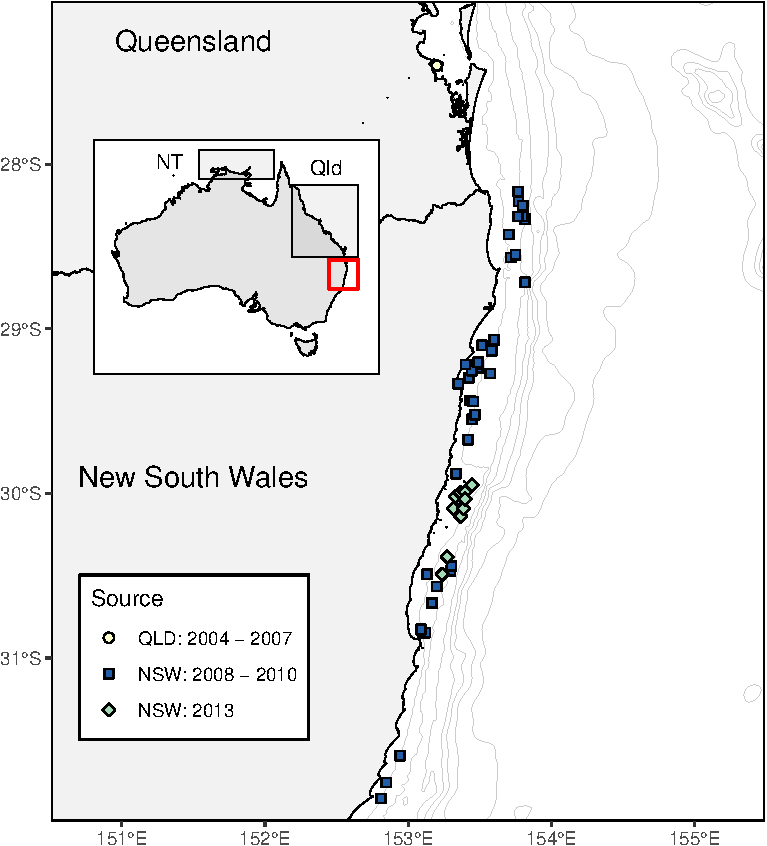
\includegraphics{/Users/avh/Documents/projects/blacktip/reports/figures_files/figure-latex/fig1-1.pdf}\\
Fig. 1

\newpage

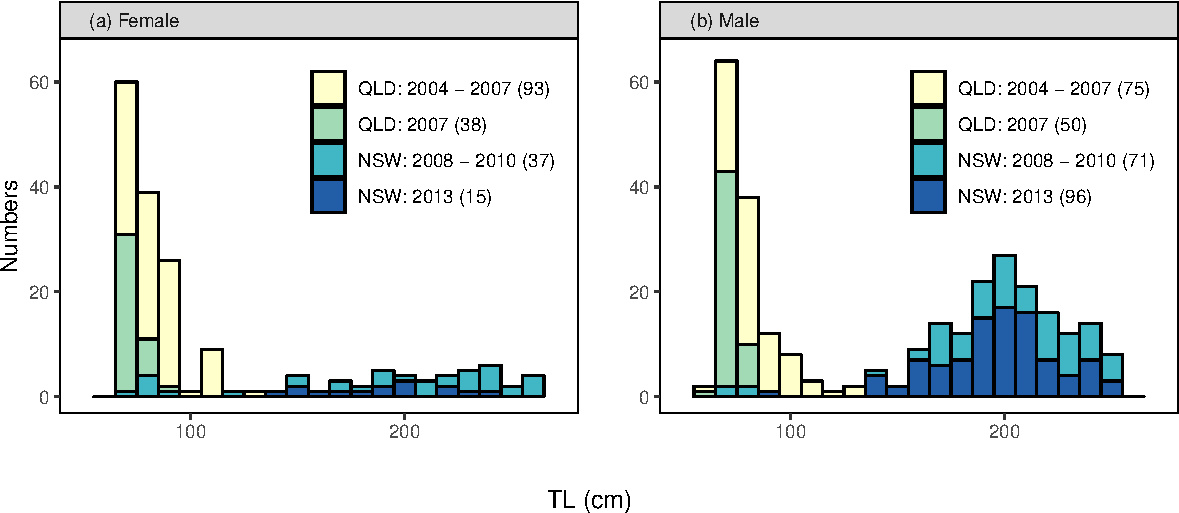
\includegraphics{/Users/avh/Documents/projects/blacktip/reports/figures_files/figure-latex/fig2-1.pdf}\\
Fig 2.

\newpage

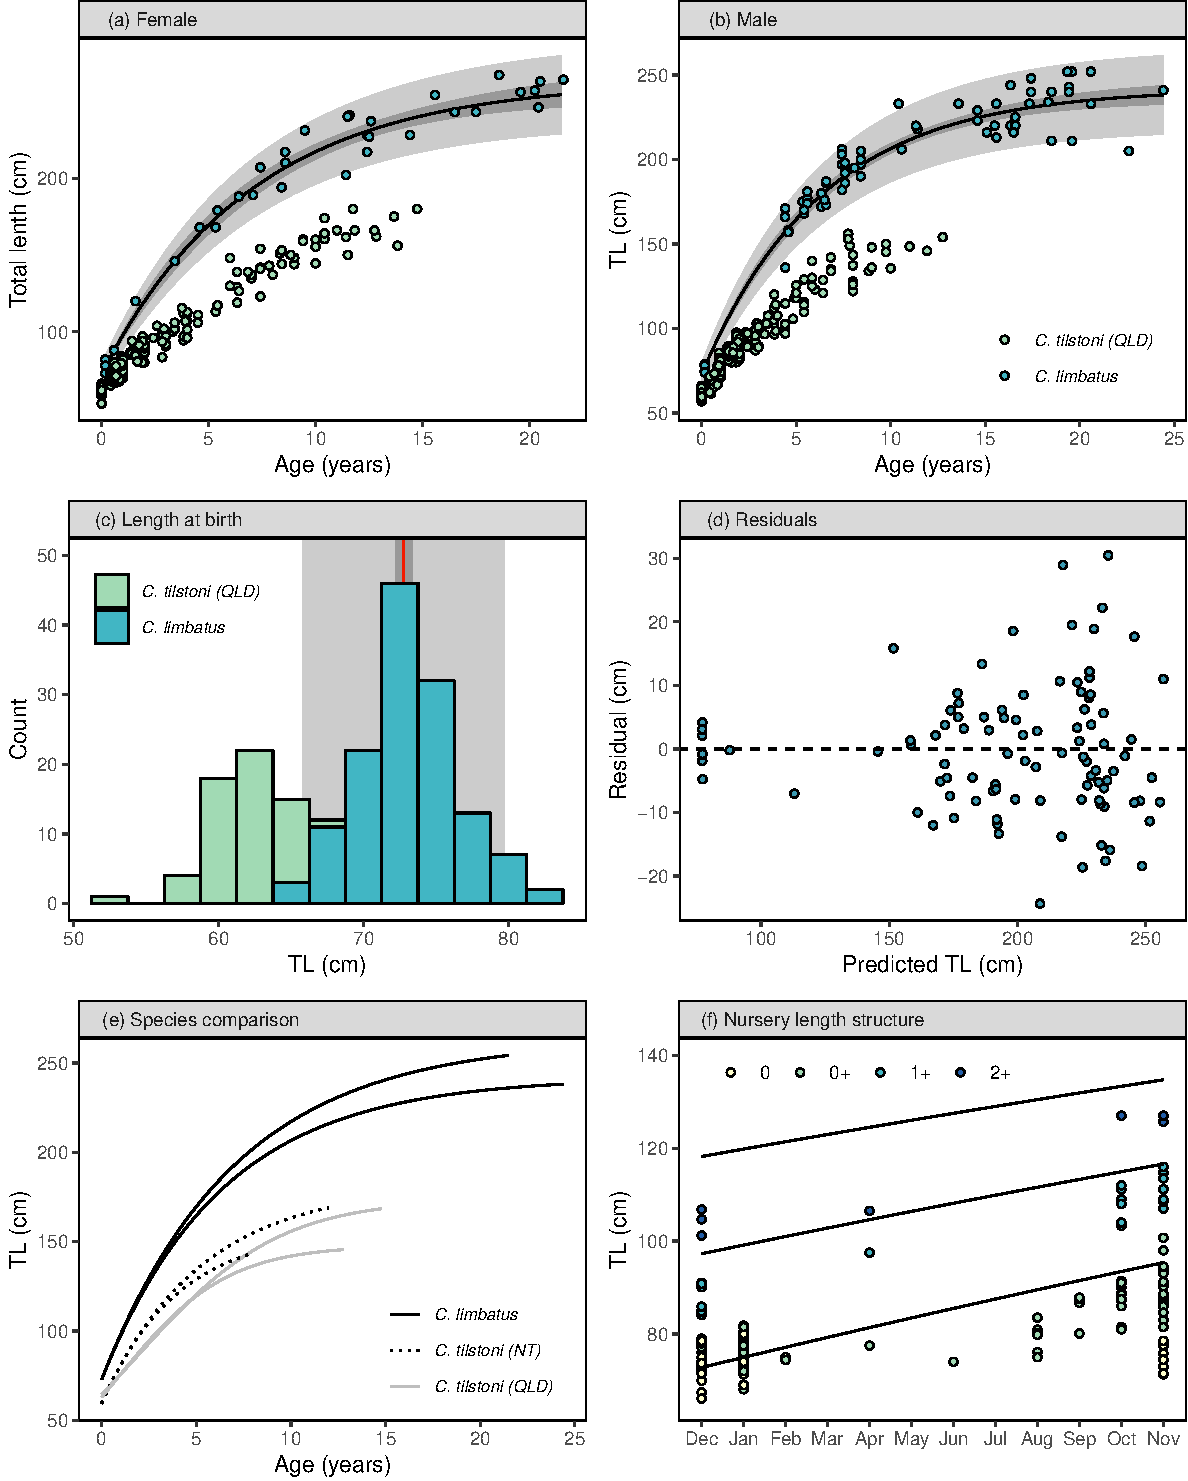
\includegraphics{/Users/avh/Documents/projects/blacktip/reports/figures_files/figure-latex/fig3-1.pdf}

Fig 3. \newpage
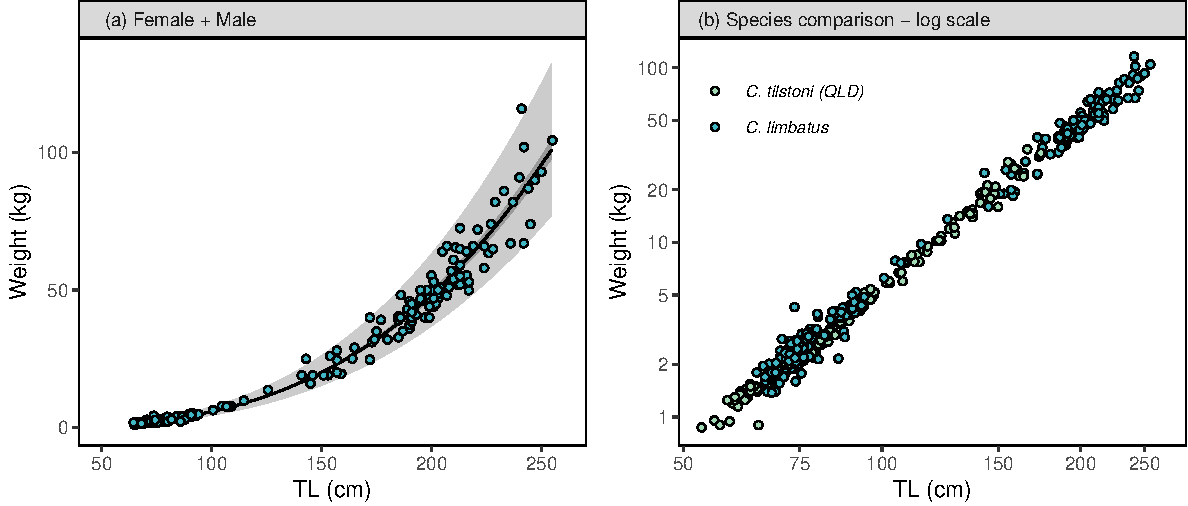
\includegraphics{/Users/avh/Documents/projects/blacktip/reports/figures_files/figure-latex/fig4-1.pdf}\\
Fig 4.

\newpage

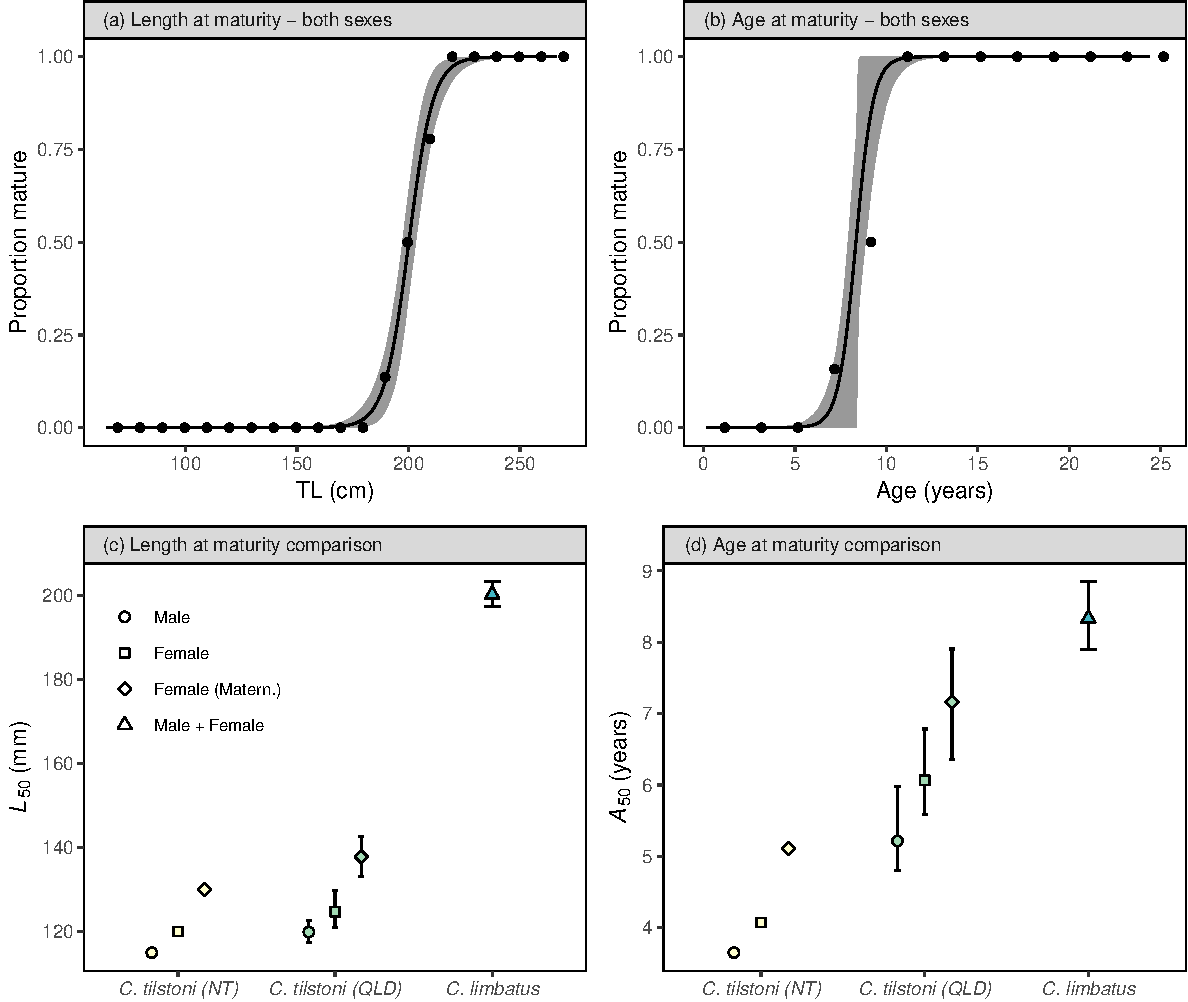
\includegraphics{/Users/avh/Documents/projects/blacktip/reports/figures_files/figure-latex/fig5-1.pdf}\\
Fig 5.

\newpage

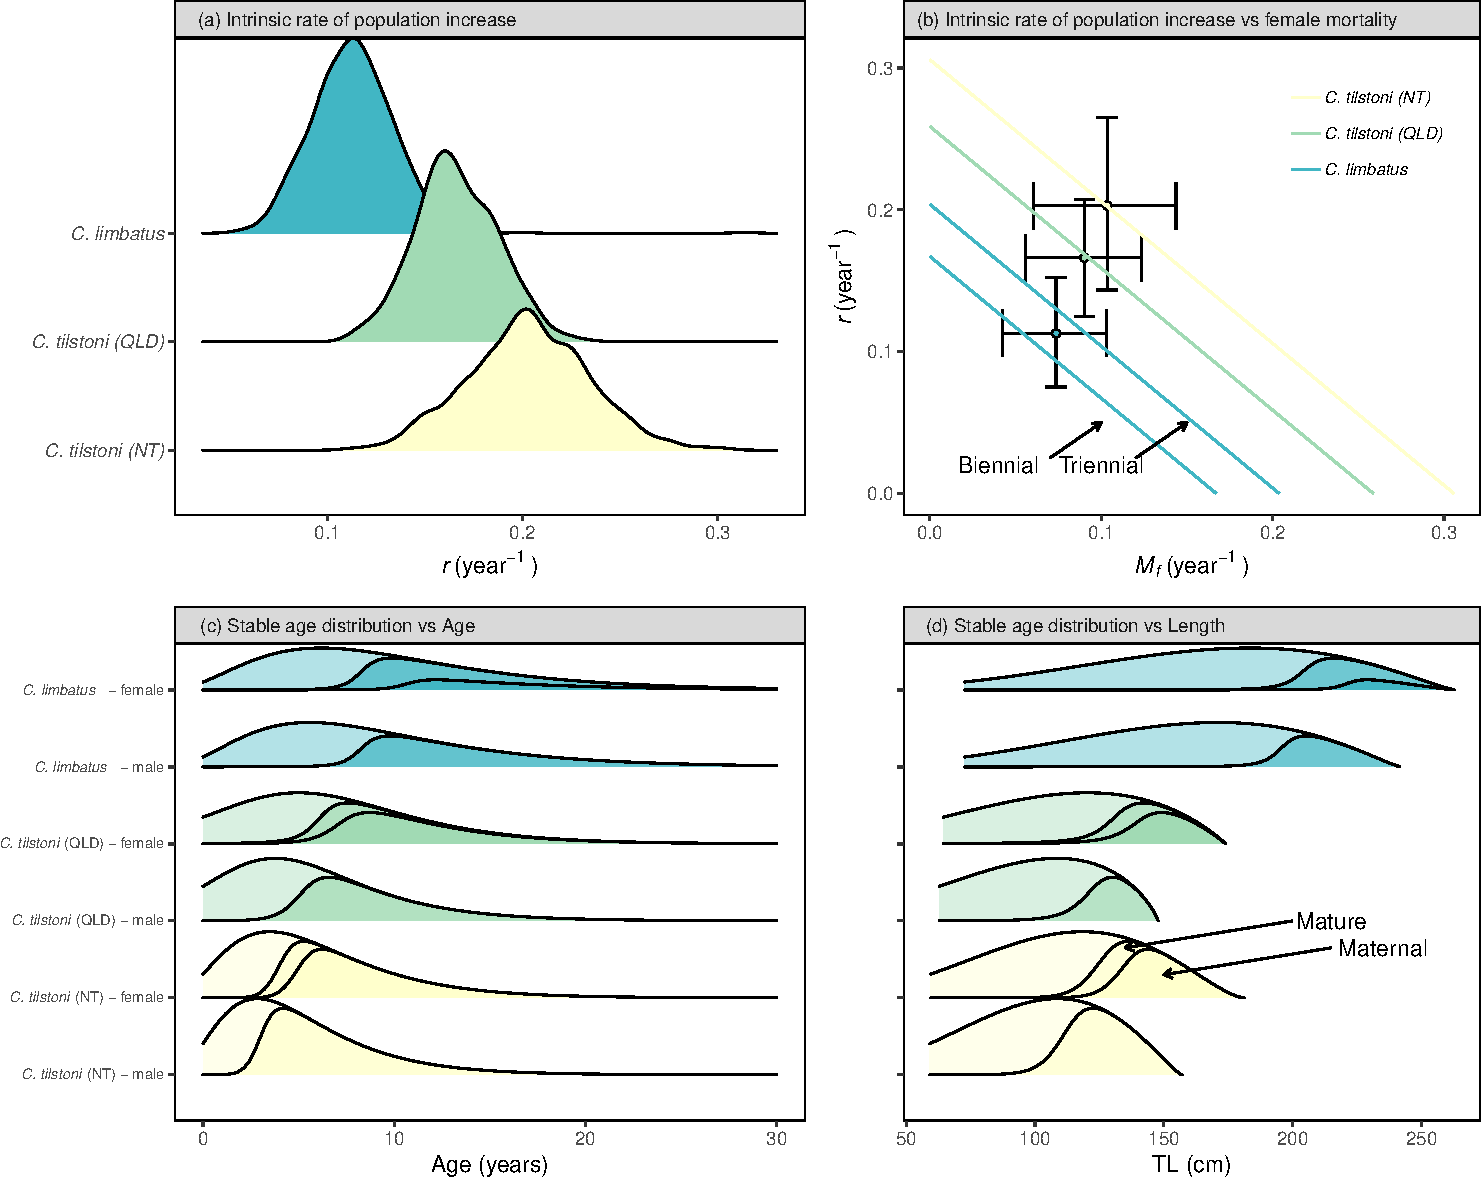
\includegraphics{/Users/avh/Documents/projects/blacktip/reports/figures_files/figure-latex/fig6-1.pdf}

Fig 6.


\end{document}
